\documentclass[english, a4paper, 10pt, headings=small, DIV11]{scrartcl}
% \VignetteIndexEntry{chondro: Vignette demonstrating example workflow using the chondro data set.}
% \VignetteKeywords{chondro, hyperSpec, cluster analysis, preprocessing, Raman, principal component analysis, PCA}
% \VignettePackage{hyperSpec}

% -*- mode: noweb; noweb-default-code-mode: R-mode; -*-
\usepackage[T1]{fontenc}
\usepackage[utf8]{inputenx}
\DeclareUnicodeCharacter{03BB}{\ensuremath{\lambda}}
\setlength{\parskip}{\medskipamount}
\setlength{\parindent}{0pt}
\usepackage{color}
\usepackage{babel}

\usepackage{fourier}
\usepackage[]{helvet}

\usepackage{array}
\usepackage{textcomp}
\usepackage{url}
\usepackage{amsmath}
\usepackage{graphicx}
\usepackage[numbers]{natbib}
\usepackage[unicode = true,
            bookmarks = true,
            bookmarksnumbered = false,
            bookmarksopen = false,
            breaklinks = false,
            backref = false,
            colorlinks = true,
            citecolor=green!50!black,        % color of links to bibli
            filecolor=blue!50!black,         % color of file links
            urlcolor=blue!50!black,          % color of external links
            linkcolor=blue!50!black          % color of internal links
           ]{hyperref}
\usepackage{hyphenat}
\usepackage{paralist}

\AtBeginDocument{
  	\setlength{\parskip}{\medskipamount}
	\setlength{\parindent}{0pt}
   \fvset{listparameters={\setlength{\topsep}{0pt}}}
   \renewenvironment{Schunk}{\vspace{0pt}\begin{small}}{\end{small}\vspace{0pt}}
   \RecustomVerbatimEnvironment{Sinput}{Verbatim}{formatcom=\small}
   \RecustomVerbatimEnvironment{Soutput}{Verbatim}{formatcom=\footnotesize}
}

% my preferred packages
\usepackage{xspace}
\usepackage{tikz}
\usepackage{subfig}
\usepackage{booktabs}

\usepackage{hyphenat}
\usepackage{fancyvrb}

\usepackage[font=footnotesize, labelfont=bf, labelsep=quad, format=plain]{caption}

\makeatletter
\@ifundefined{showcaptionsetup}{}{%
 \PassOptionsToPackage{caption=false}{subfig}}
\usepackage{subfig}
\makeatother

% fancy warning box
\newcommand{\warnbox}[3][red]{
\begin{tikzpicture}
\node [draw=#1, very thick, rectangle, rounded corners, inner sep=10pt] (box){%
    \begin{minipage}{\linewidth}
      \vspace{0.5\baselineskip}
      #3
    \end{minipage}
};
\node[fill = #1, text = white, right=5mm, rounded corners] at (box.north west)
  {\sffamily\bfseries\large #2};
\end{tikzpicture}%
}

\newcommand{\Rcode}[2][]{\texorpdfstring{\nohyphens{#1\texttt{#2}}}{#2}}
\newcommand{\Robject}[2][]{\texorpdfstring{\nohyphens{#1\texttt{#2}}}{#2}}
\newcommand{\Rcommand}[2][]{\texorpdfstring{\nohyphens{#1\texttt{#2}}}{#2}}
\newcommand{\Rfunction}[2][]{\texorpdfstring{\nohyphens{#1\texttt{#2}}}{#2}}

\newcommand{\Rfunarg}[1]{\texorpdfstring{\nohyphens{\textit{#1}}}{#1}}
\newcommand{\Rpackage}[1]{\texorpdfstring{\nohyphens{\textit{#1}}}{#1}}
\newcommand{\Rmethod}[1]{\texorpdfstring{\nohyphens{\textit{#1}}}{#1}}
\newcommand{\Rclass}[1]{\texorpdfstring{\nohyphens{\textit{#1}}}{#1}}

\newcommand{\df}{\Rclass{data.frame}\xspace}

\newcommand{\mFun}[1]{\marginpar{\scriptsize \Rfunction{#1}}}

\newcommand{\phy}{\texorpdfstring{\nohyphens{\textit{hyperSpec}}}{hyperSpec}\xspace}
\newcommand{\chy}{\Rclass{hyperSpec}\xspace}

\newcommand{\eg}{e.\,g.\xspace}
\newcommand{\ie}{i.\,e.\xspace}

\newcommand{\mum}[1]{\ensuremath{#1\;}\textmu m\xspace}
\newcommand{\rcm}[1]{\ensuremath{#1\;\mathrm{cm^{-1}}}\xspace}

\newcommand{\R}{\texorpdfstring{\texttt{R}}{R}\xspace}

\author{%
Claudia Beleites %
  \url{%
<Claudia.Beleites@chemometrix.gmbh>%
}\\
\large DIA Raman Spectroscopy Group, University of Trieste/Italy (2005\,--\,2008)\\
\large Spectroscopy $\cdot$ Imaging, IPHT, Jena/Germany (2008\,--\,2017)\\
\large ÖPV, JKI, Berlin/Germany (2017\,--\,2019)\\
\large Arbeitskreis Lebensmittelmikrobiologie und Biotechnologie, Hamburg University, Hamburg/Germany (2019\,--\,2020)\\
\large Chemometric Consulting and Chemometrix GmbH, Wölfersheim/Germany (since 2016)%
}



%\SweaveOpts{prefix.string=fig/fig}

\AtBeginDocument{
\setkeys{Gin}{width = .5\textwidth}
}

\newcommand{\mailme}{\href{mailto:Claudia Beleites <Claudia.Beleites@chemometrix.gmbh>}{\texttt{Claudia Beleites <Claudia.Beleites@chemometrix.gmbh>}}}


\hypersetup{pdftitle={Chondro},
 pdfauthor={C. Beleites},
 pdfsubject={Vignette on hyperSpec's chondro data set},
 pdfkeywords={chondro, hyperSpec, cluster analysis, preprocessing, Raman, principal component analysis, PCA}}

%\VignetteDepends{latticeExtra}
%\VignetteSuggests{akima}
\usepackage{fourier}
\usepackage[]{helvet}

\usepackage{Sweave}
\begin{document}
\Sconcordance{concordance:chondro.tex:/home/cb/Projekte/hyperSpec/Vignettes/chondro/chondro.Rnw:%
1 4 1}
\Sconcordance{concordance:chondro.tex:/home/cb/Projekte/hyperSpec/Vignettes/chondro/vignettes.defs:ofs 5:%
1 116 1 1 241 1 9 1 8 1 6}
\Sconcordance{concordance:chondro.tex:/home/cb/Projekte/hyperSpec/Vignettes/chondro/chondro.Rnw:ofs 126:%
7 10 1 1 0 15 1 1 5 61 1 1 2 1 0 1 1 15 0 1 2 1 1 1 2 4 0 1 2 1 1 1 2 4 0 1 2 22 1 1 3 2 %
0 1 1 3 0 1 3 4 0 1 3 1 0 1 2 4 0 1 2 4 1 1 2 1 0 1 1 3 0 2 2 4 0 1 2 10 1 1 2 1 0 1 1 15 %
0 1 2 1 1 1 2 4 0 1 2 5 1 1 2 1 0 1 1 3 0 1 2 12 1 1 2 1 0 1 1 3 0 1 2 15 1 1 2 1 0 1 1 3 %
0 1 2 12 1 1 2 1 0 1 3 1 0 1 3 4 0 1 2 3 1 1 2 4 0 1 2 6 1 1 3 2 0 2 1 3 0 1 2 1 4 1 2 6 %
0 1 1 1 2 1 1 3 0 1 2 3 1 1 3 2 0 1 7 8 0 1 2 3 1 1 2 1 0 4 1 3 0 1 2 2 1 1 2 4 0 1 2 26 %
1 1 2 1 0 1 1 3 0 2 2 4 0 1 2 2 1 1 2 1 0 1 1 3 0 1 2 4 1 1 2 4 0 2 2 4 0 1 2 2 1 1 2 1 0 %
2 1 3 0 1 2 9 1 1 2 1 0 1 1 3 0 1 2 19 1 1 2 1 0 1 2 4 0 1 2 14 1 1 4 6 0 1 2 2 1 1 2 1 0 %
1 1 3 0 1 4 5 0 1 2 7 1 1 13 15 0 1 2 13 1 1 2 1 0 1 1 1 2 6 1 1 4 5 0 1 2 3 1 1 -125 30 %
0 1 2 1 127 1 1}

\title{Raman Spectra of Chondrocytes in Cartilage:\\
\Rpackage{hyperSpec}'s \texttt{chondro} data set }
\maketitle

\warnbox{Reproducing this vignette}{ The data set and source file of this vignette are available at \Rpackage{hyperSpec}'s github page at 
 \url{https://github.com/cbeleites/hyperSpec/blob/master/Vignettes/chondro/chondro.Rnw} and 
  \url{https://github.com/cbeleites/hyperSpec/tree/master/Vignettes/fileio/txt.Renishaw/chondro.txt} (ca. 31 MB). The .Rnw looks for \texttt{rawdata/chondro.txt}, so please save the data file in subdirectory  \texttt{rawdata} of your working directory.

  In order to reproduce the examples by typing in the commands, have a look at the definitions of
  color palettes used in this document are defined in \texttt{vignettes.defs}. Also, the package \phy
  needs to be loaded first via \Rcode{library (hyperSpec)}.  }

\tableofcontents


\section{Introduction}

This vignette describes the \Robject{chondro} data set. It shows a complete data analysis work flow
on a Raman map demonstrating frequently needed preprocessing methods
\begin{compactitem}
\item baseline correction
\item normalization
\item smoothing / interpolating spectra
\item preprocessing the spatial grid
\end{compactitem}
and other basic work techniques
\begin{compactitem}
\item plotting spectra
\item plotting false color maps
\item cutting the spectral range,
\item selecting (extracting) or deleting spectra, and
\item \emph{aggregating} spectra (e.g. calculating cluster mean spectra).
\end{compactitem}
The chemometric methods used are
\begin{compactitem}
\item Principal Component Analysis (PCA) and
\item Hierarchical Cluster Analysis,
\end{compactitem}
showing how to use data analysis procedures provided by R and other
packages.


\section{The Data Set}
\begin{figure}
\noindent 
\begin{centering}
  \includegraphics[width=0.5\textwidth]{080606d-flip-ausw}
  \par
\end{centering}
\caption{\label{fig:vis-all}Microphotograph of the cartilage section. The frame indicates the
  measurement area (\mum{35~\times~25}).}
\end{figure}

Raman spectra of a cartilage section were measured on each point of a grid, resulting in a so-called
\emph{Raman map}. Figure~\ref{fig:vis-all} shows a microscope picture of the measured area and its
surroundings.

The measurement parameters were:
\begin{compactdesc}
\item [Excitation wavelength:] 633 nm
\item [Exposure time:] 10 s per spectrum
\item [Objective:] 100$\times$, NA 0.85
\item [Measurement grid:] 35 $\times$ 25 \mum{}, 1 \mum{} step size
\item [Spectrometer:] Renishaw InVia
\end{compactdesc}

\section{Data Import}
Renishaw provides a converter to export their proprietary data in a so-called long format ASCII
file. Raman maps are exported having four columns, \emph{y}, \emph{x}, \emph{raman shift}, and
\emph{intensity}.  \Rpackage{hyperSpec} comes with a function to import such files,
\Rfunction{read.txt.Renishaw}. The function assumes a map as default, but can also handle single
spectra (\Rcode{data = \textquotedbl{}spc\textquotedbl{}}), time series (\Rcode{data =
  \textquotedbl{}ts\textquotedbl{}}), and depth profiles (\Rcode{data =
\textquotedbl{}depth\textquotedbl{}}).  In addition, large files may be processed in chunks. In order
to speed up the reading \Rfunction{read.txt.Renishaw} does not allow missing values, but it does work
with \Rcode{NA}.
\begin{Schunk}
\begin{Sinput}
> chondro <- read.txt.Renishaw ("rawdata/chondro.txt", data = "xyspc")
> chondro
\end{Sinput}
\begin{Soutput}
hyperSpec object
   875 spectra
   4 data columns
   1272 data points / spectrum
wavelength: Delta * tilde(nu)/cm^-1 [numeric] 601.62 602.66 ... 1802.2 
data:  (875 rows x 4 columns)
   1. y: y/(mu * m) [numeric] -4.77 -4.77 ... 19.23 
   2. x: x/(mu * m) [numeric] -11.55 -10.55 ... 22.45 
   3. spc: I / a.u. [matrix1272] 501.72 518.53 ... 151.92 + NA
   4. filename: filename [character] rawdata/chondro.txt rawdata/chondro.txt ... rawdata/chondro.txt 
\end{Soutput}
\end{Schunk}

To get an overview of the spectra (figure~\ref{fig:raw:a}):
\begin{Schunk}
\begin{Sinput}
> plot (chondro, "spcprctl5")
\end{Sinput}
\end{Schunk}

A mean intensity map (figure~\ref{fig:raw:b}) is produced by:
\begin{Schunk}
\begin{Sinput}
> plotmap (chondro, func.args = list (na.rm = TRUE), col.regions = seq.palette (20))
\end{Sinput}
\end{Schunk}
\Rfunction{plotmap} applies a function to squeeze all spectral intensities into a summary characteristic for the whole spectrum. This function defaults to the \Rfunction{mean}. Further arguments that should be handed to this function can be given in list \Rfunarg{func.args}. As the raw data contains \Rcode{NA}s due to deleting cosmic ray spikes, this argument is needed here.
\begin{figure}[tbh]
\subfloat[\label{fig:raw:a}The raw spectra: median, 16\textsuperscript{th} and 84\textsuperscript{th}, and 5\textsuperscript{th} and 95\textsuperscript{th} percentile
spectra.]{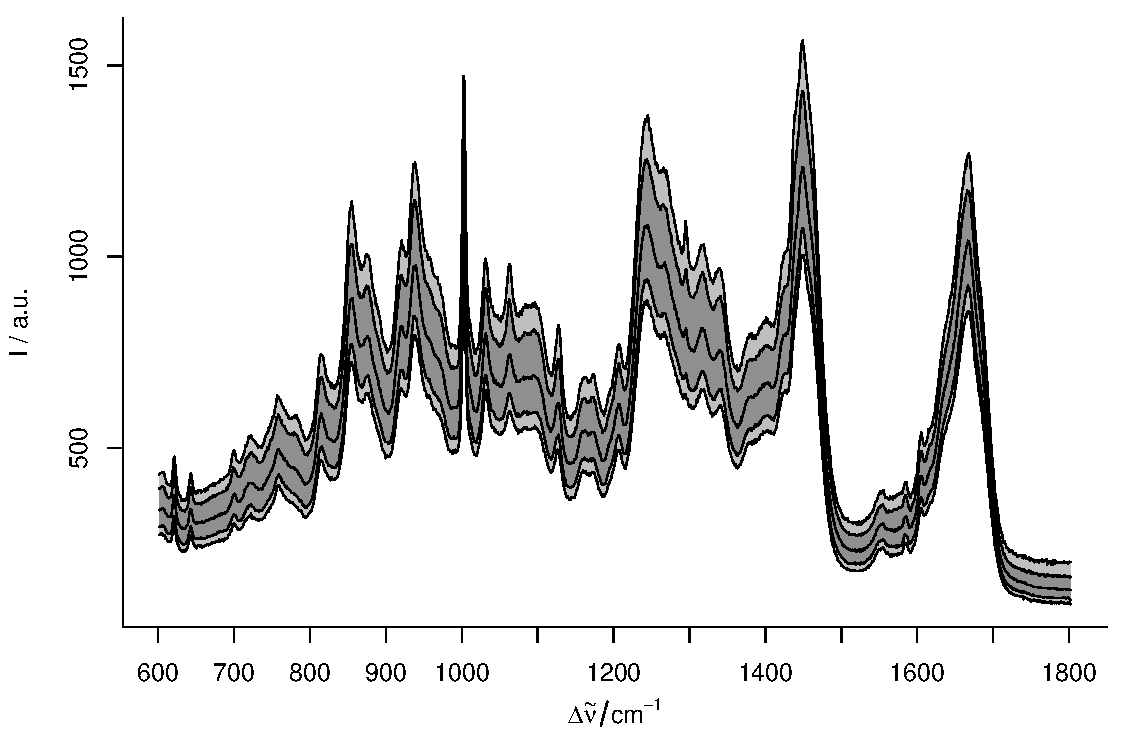
\includegraphics[width=0.5\textwidth]{chondro-fig--rawspc}}
\subfloat[\label{fig:raw:b}The sum intensity of the raw spectra.]{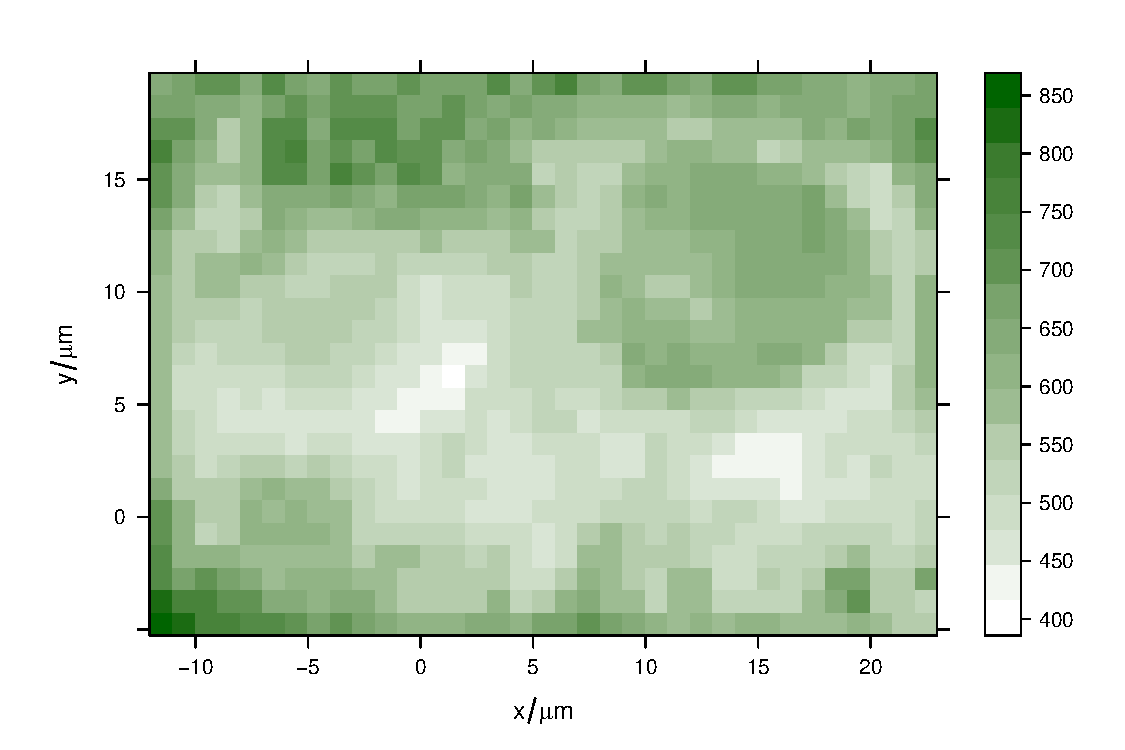
\includegraphics[width=0.5\textwidth]{chondro-fig--rawmap}}
\caption{\label{fig:raw} The raw spectra.}
\end{figure}

\section{Preprocessing}
As usual in Raman spectroscopy of biological tissues, the spectra need some preprocessing.

\subsection{Aligning the Spatial Grid} 

The spectra were acquired on a regular square grid of measurement positions over the sample. \chy
however does not store the data on this grid but rather stores the position where the spectra were
taken. This allows more handling of irregular point patterns, and of sparse measurements where not a
complete (square) is retained but only few positions on this grid.

Occasionally, numeric or rounding errors will lead to seemingly irregular spacing of the data
points. This is most obvious in false-colour maps of the sample (fig.~{fig:raw:b}), as
\Rcode{plotmap} by default uses \Rcode{panel.levelplot.raster} which assumes a regular grid is
underlying the data. The symptoms are warnings ``'x' values are not equispaced; output may be wrong''
and white stripes in the false colour map (fig~\ref{fig:irregular:a}) which occur even thought the points are almost at their correct place (fig~\ref{fig:irregular:b})
\begin{Schunk}
\begin{Sinput}
> ## disturb a few points
> chondro$x [500] <- chondro$x [500] + rnorm (1, sd = 0.01)
> chondro$y [660] <- chondro$y [660] + rnorm (1, sd = 0.01)
\end{Sinput}
\end{Schunk}
\begin{Schunk}
\begin{Sinput}
> plotmap (chondro, col.regions = seq.palette (20))
\end{Sinput}
\end{Schunk}
\begin{Schunk}
\begin{Sinput}
> require ("latticeExtra")
> plotmap (chondro, col.regions = seq.palette (20), panel = panel.levelplot.points,
+          col = NA, pch = 22, cex = 1.9)
\end{Sinput}
\end{Schunk}

Such slight rounding errors can be corrected by \Rcode{fitraster} or \Rcode{makeraster}.
\Rcode{fitraster} needs the step size of the raster and a starting coordinate, whereas
\Rcode{makeraster} tries to guess these parameters for \Rcode{fitraster}. As long as just a few
points are affected by rounding errors, \Rcode{makeraster} works fine:
\begin{Schunk}
\begin{Sinput}
> chondro$x <- fitraster (chondro$x)$x
> chondro$y <- fitraster (chondro$y)$x
\end{Sinput}
\end{Schunk}
the result is shown in figure~\ref{fig:irregular:c}.
\begin{Schunk}
\begin{Sinput}
> plotmap (chondro, col.regions = seq.palette (20))
\end{Sinput}
\end{Schunk}

\begin{figure}[tbh]
\subfloat[\label{fig:irregular:a}Off-grid points cause stripes]{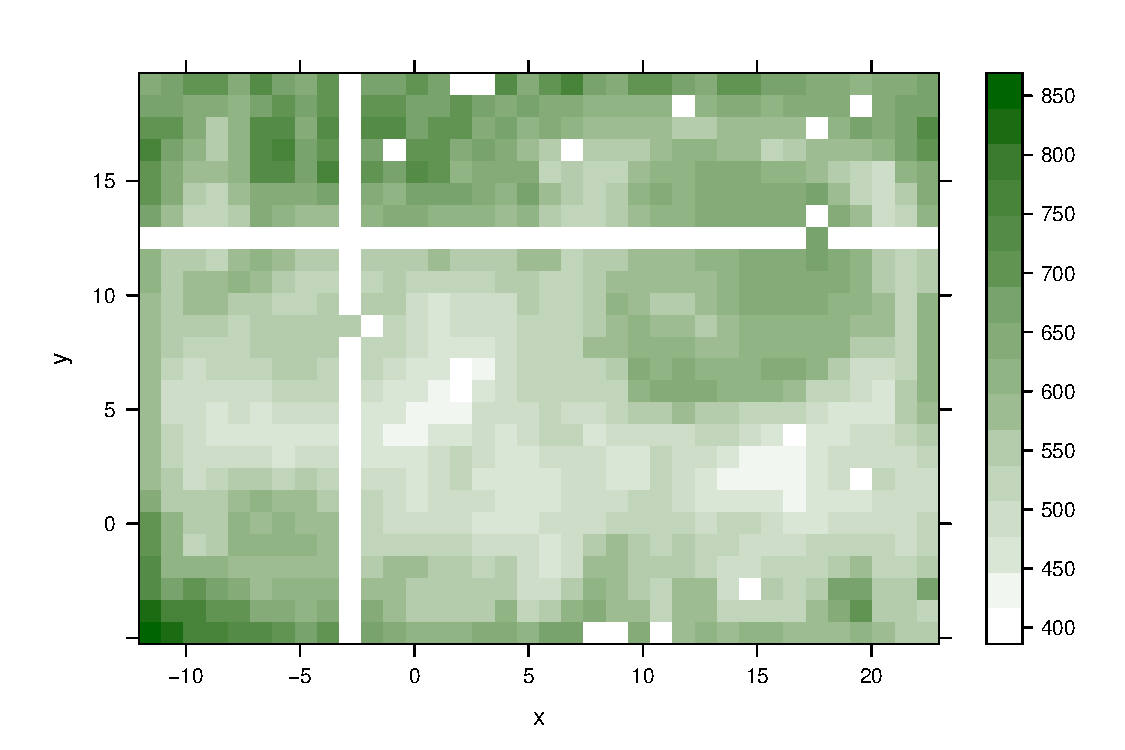
\includegraphics[width=0.3\textwidth]{chondro-fig--irregular-grid}}
\subfloat[\label{fig:irregular:b}Slightly wrong coordinages]{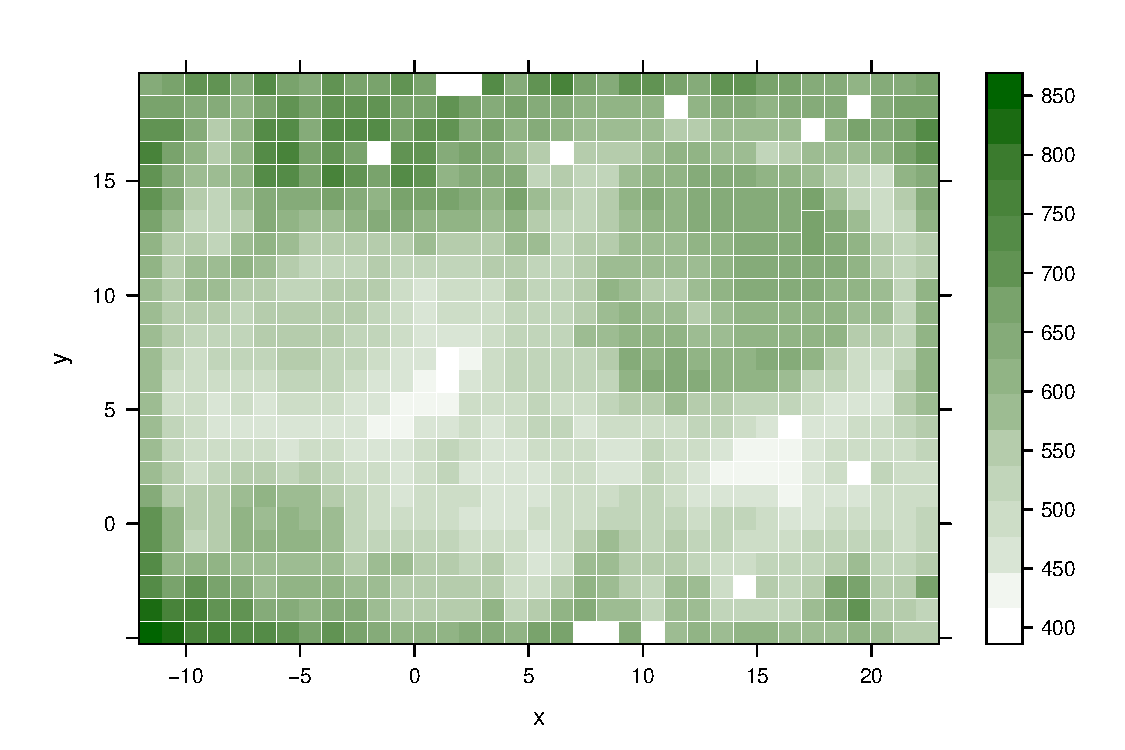
\includegraphics[width=0.3\textwidth]{chondro-fig--irregular-pts}}
\subfloat[\label{fig:irregular:c}Corrected grid]{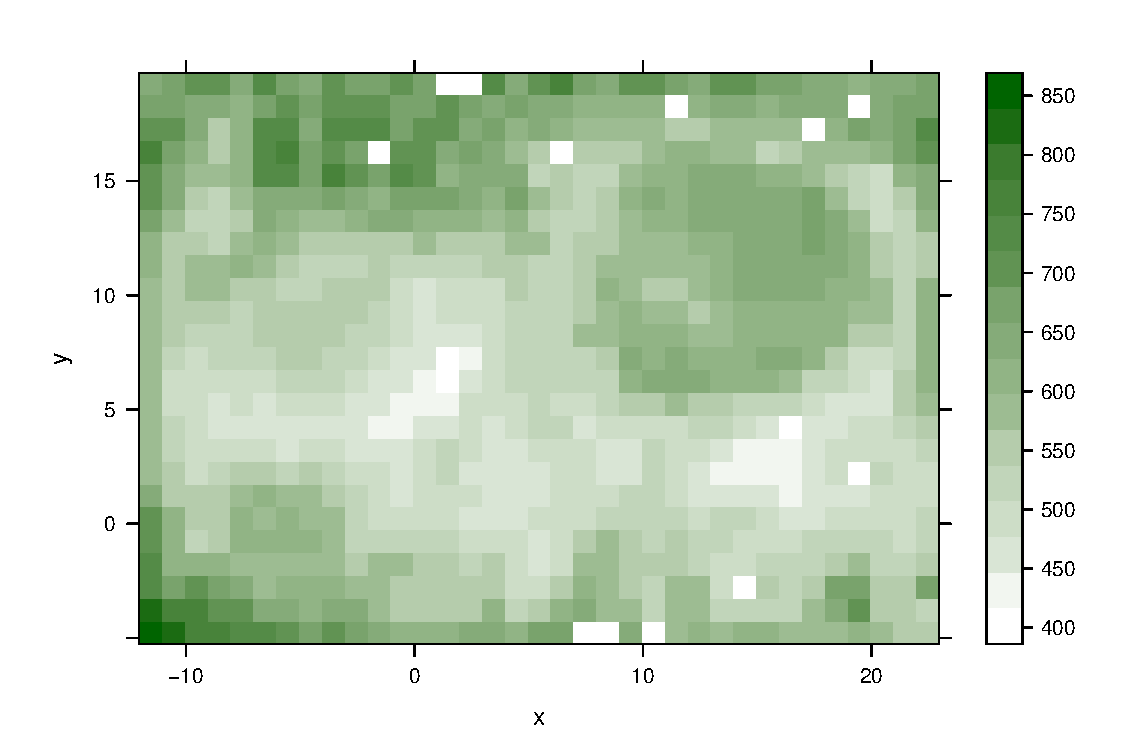
\includegraphics[width=0.3\textwidth]{chondro-fig--irregular-corr}}
\caption{\label{fig:pointerror} Rounding erros in the point coordinates of lateral measurement grid.}
\end{figure}

\subsection{Spectral Smoothing}
As the overview shows that the spectra contain \Rcode{NA}s (from cosmic spike removal that was done previously), the first step is to remove these. Also, the wavelength axis of the raw spectra is not evenly spaced (the data points are between 0.85 and 1\,\rcm{} apart from each other). Furthermore, it would be good to trade some spectral resolution for higher signal to noise ratio. All three of these issues are tackled by interpolating and smoothing of the wavelength axis by \Rfunction{spc.loess}. The resolution is to be reduced to \rcm{8}, or \rcm{4} data point spacing.

\begin{Schunk}
\begin{Sinput}
> chondro <- spc.loess (chondro, seq (602, 1800, 4))
> chondro
\end{Sinput}
\begin{Soutput}
hyperSpec object
   875 spectra
   4 data columns
   300 data points / spectrum
wavelength: Delta * tilde(nu)/cm^-1 [numeric] 602 606 ... 1798 
data:  (875 rows x 4 columns)
   1. y: y [numeric] -4.77 -4.77 ... 19.23 
   2. x: x [numeric] -11.55 -10.55 ... 22.45 
   3. spc: I / a.u. [matrix300] 517.03 499.77 ... 168.04 
   4. filename: filename [character] rawdata/chondro.txt rawdata/chondro.txt ... rawdata/chondro.txt 
\end{Soutput}
\end{Schunk}

The spectra are now the same as in the data set \Robject{chondro}. However, the data set also contains the clustering results (see at the very end of this document). They are stored for saving as the distributed demo data:
\begin{Schunk}
\begin{Sinput}
> spectra.to.save <- chondro
\end{Sinput}
\end{Schunk}

\subsection{Baseline Correction}
The next step is a linear baseline correction. \Rfunction{spc.fit.poly.below}
tries to automatically find appropriate support points for polynomial
baselines. The default is a linear baseline, which is appropriate
in our case:
\begin{Schunk}
\begin{Sinput}
> baselines <- spc.fit.poly.below (chondro)
> chondro <- chondro - baselines
\end{Sinput}
\end{Schunk}

\begin{figure}[tbh]
\subfloat[\label{fig:bl-bl} The spectra after smoothing, baseline correction, and normalization.]{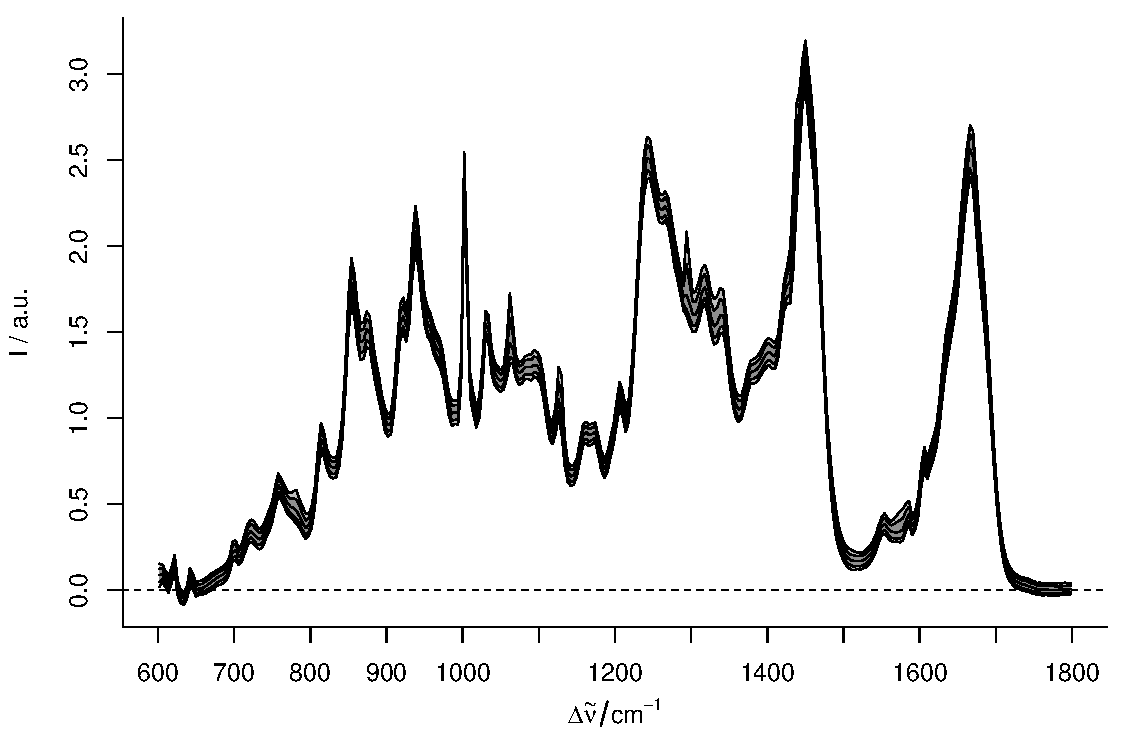
\includegraphics[width=0.4\textwidth]{chondro-fig--norm}}\quad%
\subfloat[\label{fig:bl:perc} The spectra after subtracting the 5\textsuperscript{th} percentile spectrum.]{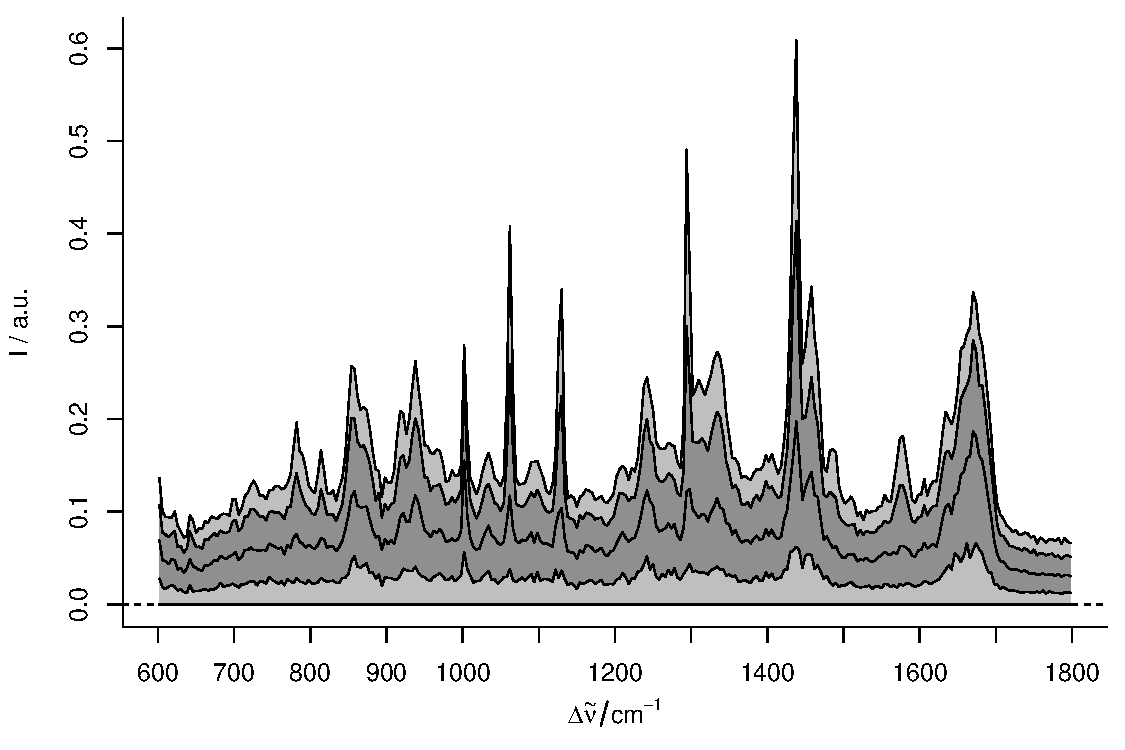
\includegraphics[width=0.4\textwidth]{chondro-fig--perc}}
\caption{\label{fig:bl}The preprocessed spectra.}
\end{figure}



\subsection{Normalization}

As the spectra are quite similar, area normalization should work well:.

\begin{Schunk}
\begin{Sinput}
> chondro <- chondro / rowMeans (chondro)
> plot (chondro, "spcprctl5")
\end{Sinput}
\end{Schunk}

Note that normalization effectively cancels the information of one variate (wavelength), it
introduces a collinearity. If needed, this collinearity can be broken by removing one of the variates
involved in the normalization. Note that the \Robject{chondro} object shipped with \phy set has
multiple collinearities as only the first 10 principal components are shipped (see below).

For the results of these preprocessing steps, see figure~\ref{fig:bl-bl}.

\subsection{Subtracting the Overall Composition}

The spectra are very homogeneous, but I'm interested in the differences
between the different regions of the sample. Subtracting the minimum
spectrum cancels out the matrix composition that is common to all spectra.
But the minimum spectrum also picks up a lot of noise. So instead,
the 5\textsuperscript{th} percentile spectrum is subtracted:

\begin{Schunk}
\begin{Sinput}
> chondro <- chondro - quantile (chondro, 0.05)
> plot (chondro, "spcprctl5")
\end{Sinput}
\end{Schunk}

The resulting data set is shown in figure~\ref{fig:bl:perc}. Some
interesting differences start to show up: there are distinct lipid
bands in some but not all of the spectra.


\subsection{Outlier Removal by Principal Component Analysis (PCA)}

PCA is a technique that decomposes the data into scores and loadings
(virtual spectra). It is known to be quite sensitive to outliers. Thus,
I use it for outlier detection. The resulting scores and loadings
are put again into \Rclass{hyperSpec} objects by \Rfunction{decomposition}:

\begin{Schunk}
\begin{Sinput}
> pca <- prcomp (chondro, center = TRUE)
> scores <- decomposition (chondro, pca$x, label.wavelength = "PC",
+                          label.spc = "score / a.u.")
> loadings <- decomposition (chondro, t(pca$rotation), scores = FALSE,
+                            label.spc = "loading I / a.u.")
\end{Sinput}
\end{Schunk}

Plotting the scores of each PC against all other gives a good idea
where to look for outliers.

\begin{Schunk}
\begin{Sinput}
> pairs (scores [[,,1:20]], pch = 19, cex = 0.5)
\end{Sinput}
\end{Schunk}

Now the spectra can be found either by plotting two scores against
each other (by \Rfunction{plot}) and identifying with \Rfunction{identify},
or they can be identified in the score map by \Rfunction{map.identify}.
There is also a function to identify spectra in a spectra plot, \Rfunction{spc.identify},
which could be used to identify principal components that are heavily influenced \eg by cosmic ray spikes.

\begin{Schunk}
\begin{Sinput}
> ## omit the first 4 PCs
> out <- map.identify (scores [,,5])
> out <- c (out, map.identify (scores [,,6]))
> out <- c (out, map.identify (scores [,,7]))
\end{Sinput}
\end{Schunk}


\begin{Schunk}
\begin{Sinput}
> out
\end{Sinput}
\begin{Soutput}
[1] 105 140 216 289  75  69
\end{Soutput}
\begin{Sinput}
> outcols <- c ("red", "blue", "#800080", "orange", "magenta", "brown")
> cols <- rep ("black", nrow(chondro))
> cols [out] <- outcols
\end{Sinput}
\end{Schunk}

We can check our findings by comparing the spectra to the bulk of
spectra (figure~\ref{PCA:b}):

\begin{Schunk}
\begin{Sinput}
> plot(chondro[1], plot.args = list (ylim = c (1, length (out) + .7)),
+ 		 lines.args = list(  type = "n"))
> for (i in seq (along = out)){
+    plot(chondro, "spcprctl5", yoffset = i, add = TRUE, col = "gray")
+    plot (chondro [out[i]], yoffset = i, col = outcols[i] , add = TRUE,
+    			lines.args = list (lwd = 2))
+    text (600, i + .33, out [i])
+ }
\end{Sinput}
\end{Schunk}

and also by looking where these spectra appear in the scores \Rfunction{pairs}
plot (figure~\ref{PCA:a}):

\begin{Schunk}
\begin{Sinput}
> png ("chondro-fig--pca-pairs2.png", width = 500, height = 500)
> pch <- rep (46L, nrow (chondro))
> pch [out] <- 19L
> pairs (scores [[,,1:7]], pch = pch, cex = 1, col = cols)
> dev.off ()
\end{Sinput}
\end{Schunk}

Finally, the outliers are removed:

\begin{Schunk}
\begin{Sinput}
> chondro <- chondro [- out]
\end{Sinput}
\end{Schunk}

%
\begin{figure}[tbh]
\subfloat[\label{PCA:b}The suspected outlier spectra.]{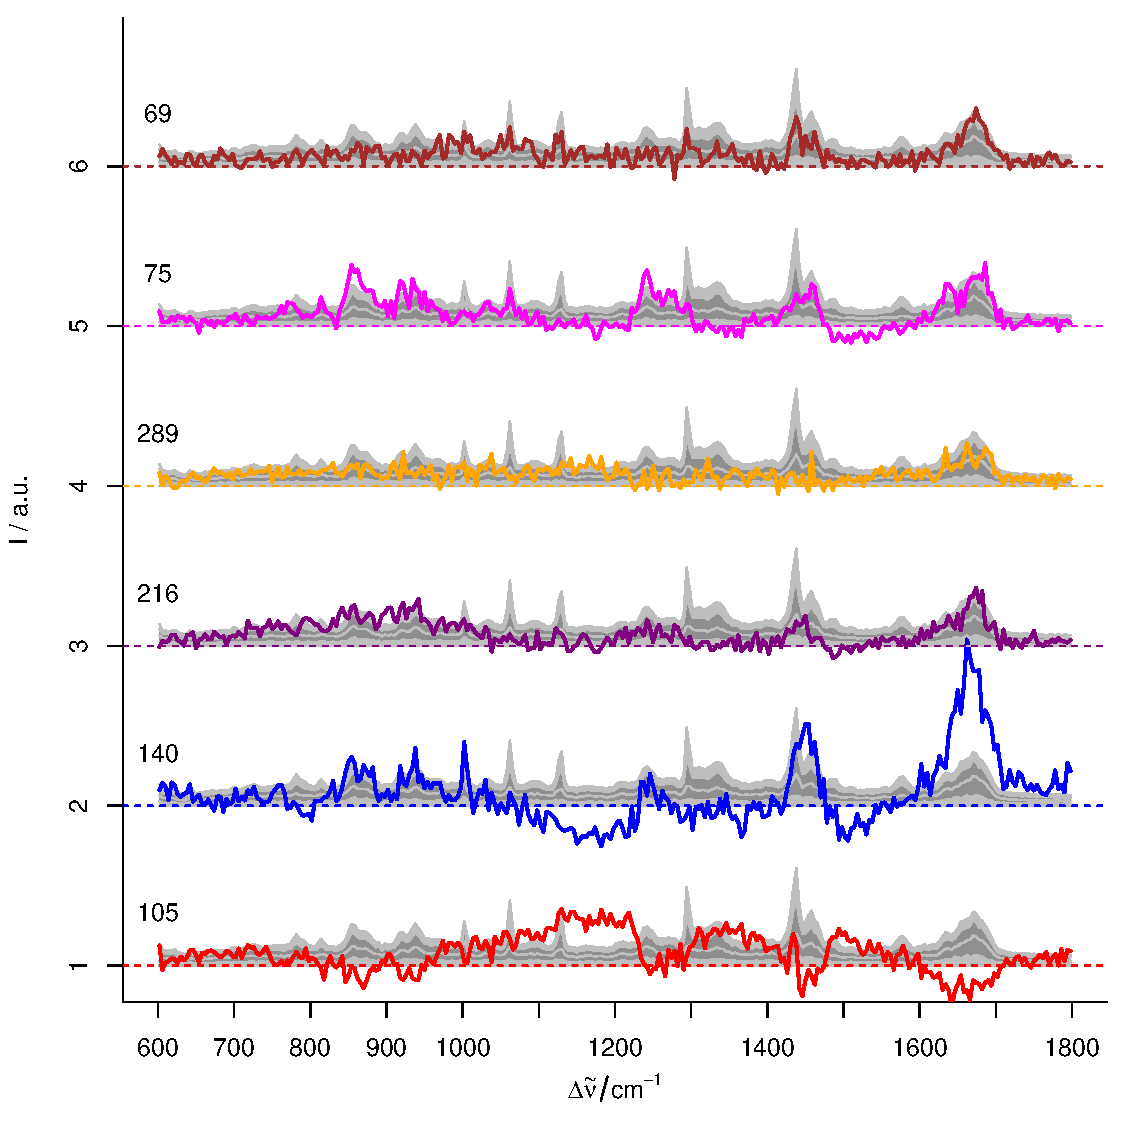
\includegraphics[width=0.495\textwidth]{chondro-fig--pca-outspc}}
\subfloat[\label{PCA:a}\Rfunction{pairs} plot of the first 7 scores.]{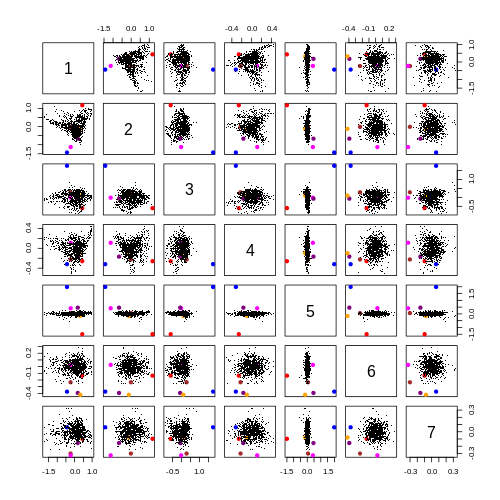
\includegraphics[width=0.495\textwidth]{chondro-fig--pca-pairs2}}%
\end{figure}



\section{Hierarchical Cluster Analysis (HCA)}

HCA merges objects according to their (dis)similarity into clusters. The result is
a dendrogram, a graph stating at which level two objects are similar
and thus grouped together.

The first step in HCA is the choice of the distance. The R function
\Rfunction{dist} offers a variety of distance measures to be computed.
The so-called \textsc{Pearson} distance \global\long\def\COR{COR}
$D^2_{Pearson}=\frac{1-\COR\left(X\right)}{2}$
is popular in data analysis of vibrational spectra and is provided
by \phy's \Rfunction{pearson.dist} function.

Also for computing the dendrogram, a number of choices are available.
Here we choose \textsc{Ward}'s method, and, as it uses \textsc{Euclid}ean
distance for calculating the dendrogram, \textsc{Euclid}ean distance
also for the distance matrix :

\begin{Schunk}
\begin{Sinput}
> dist <- dist (chondro)
> dendrogram <- hclust (dist, method = "ward.D")
\end{Sinput}
\end{Schunk}

\begin{Schunk}
\begin{Sinput}
> plot (dendrogram)
\end{Sinput}
\end{Schunk}

In order to get clusters, the dendrogram is cut at a level specified
either by height or by the number of clusters.
\begin{Schunk}
\begin{Sinput}
> chondro$clusters <- as.factor (cutree (dendrogram, k = 3))
> cols <- c ("dark blue", "orange", "#C02020")
\end{Sinput}
\end{Schunk}
The result for $k$= 3 clusters is plotted as a map (figure~\ref{fig:clustmap}). If the color-coded
variate (left hand side of the formula) is a factor, the legend bar does not show intermediate
colors, and \chy's \Rfunction{levelplot} method uses the levels of the factor for the legend.

Thus  meaningful names are assigned
\begin{Schunk}
\begin{Sinput}
> levels (chondro$clusters) <- c ("matrix", "lacuna", "cell")
\end{Sinput}
\end{Schunk}
and the cluster membership map is plotted:
\begin{Schunk}
\begin{Sinput}
> print (plotmap (chondro, clusters ~ x * y, col.regions = cols))
\end{Sinput}
\end{Schunk}

The cluster membership can also be marked in the dendrogram:

\begin{Schunk}
\begin{Sinput}
> par (xpd = TRUE)                        # allow plotting the markers into the margin
> plot (dendrogram, labels = FALSE, hang = -1)
> mark.dendrogram (dendrogram, chondro$clusters, col = cols)
\end{Sinput}
\end{Schunk}

Figure~\ref{fig:dend} shows the dendrogram and \ref{fig:clustmap}
the resulting cluster map. The three clusters correspond to the cartilage
matrix, the lacuna and the cells. The left cell is destroyed and its
contents are leaking into the matrix, while the right cells looks
intact.

We can plot the cluster mean spectra $\pm$
1 standard deviation using \Rfunction{aggregate} (see figure~\ref{fig:clustmeans}):

\begin{Schunk}
\begin{Sinput}
> cluster.means <- aggregate (chondro, chondro$clusters, mean_pm_sd)
> plot (cluster.means, stacked = ".aggregate", fill = ".aggregate", col = cols)
\end{Sinput}
\end{Schunk}

%
\begin{figure}[tbh]
\subfloat[\label{fig:dend} The dendrogram.]{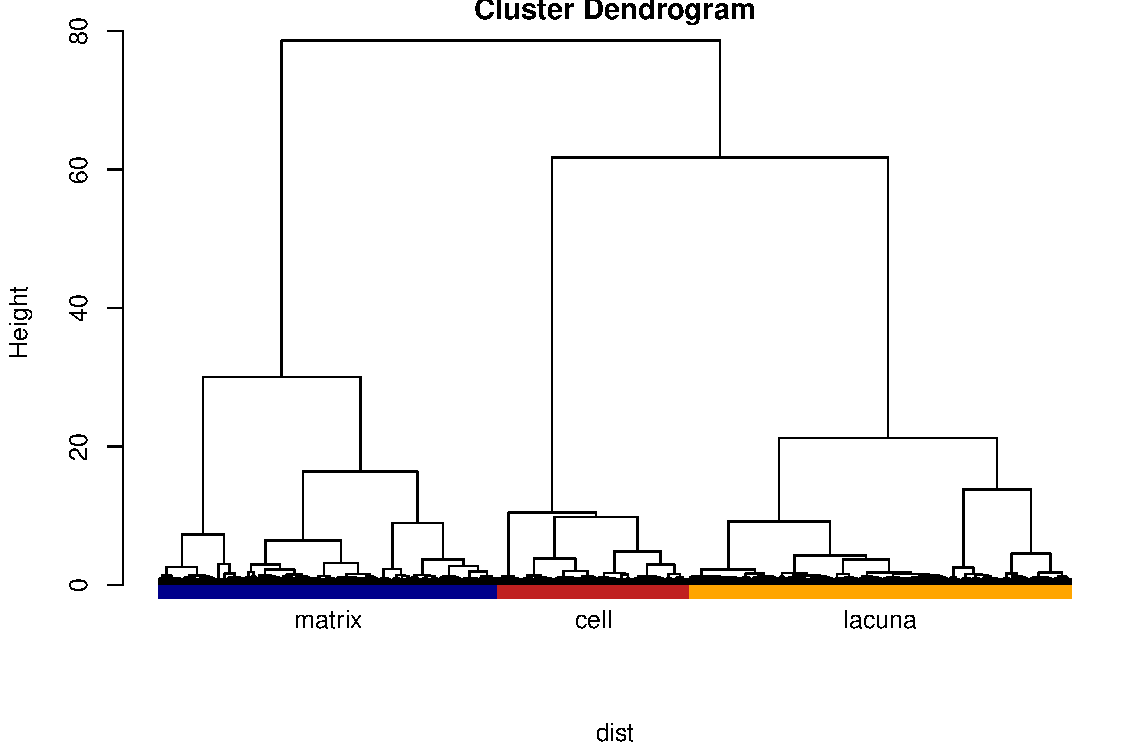
\includegraphics[width=0.495\textwidth]{chondro-fig--dend}}\subfloat[\label{fig:clustmap} The cluster map for $k=3$ clusters.]{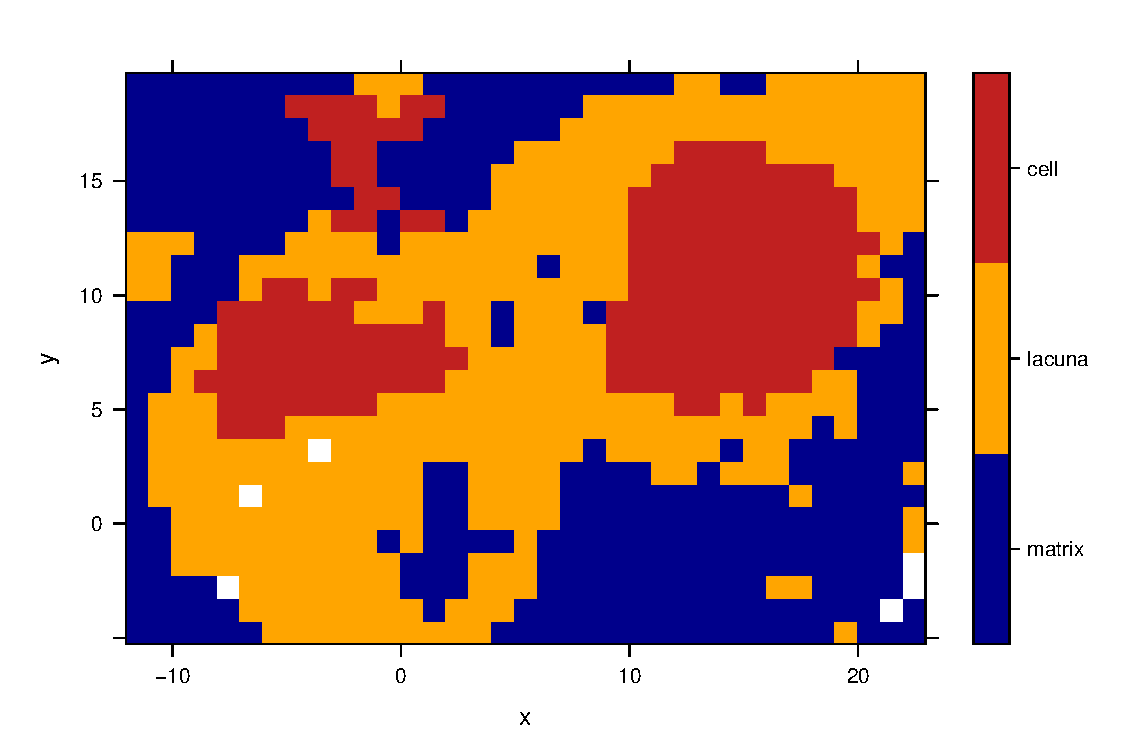
\includegraphics[width=0.495\textwidth]{chondro-fig--clustmap}}\caption{Hierarchical cluster analysis.}
\end{figure}
\begin{figure}[tbh]
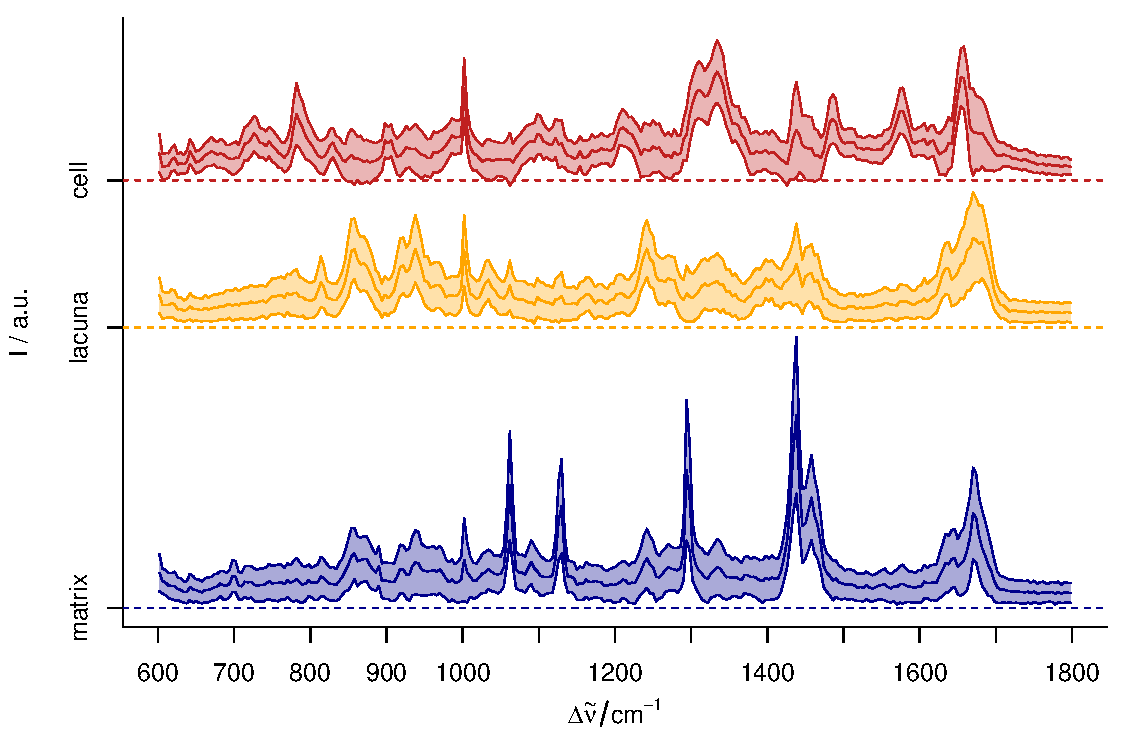
\includegraphics[width=0.495\textwidth]{chondro-fig--clustmeans}
\caption{\label{fig:clustmeans} The cluster mean $\pm$ 1 standard deviation
spectra. The blue cluster shows distinct lipid bands, the yellow cluster
collagen, and the red cluster proteins and nucleic acids.}
\end{figure}

\section{Plotting a False-Colour Map of Certain Spectral Regions}

\Rclass{hyperSpec} comes with a sophisticated interface for specifying
spectral ranges. Expressing things like 1000~cm\textsuperscript{-1}
$\pm$~1 data points is easily possible. Thus, we can have a fast
look at the nucleic acid distribution, using the DNA bands at 728,
782, 1098, 1240, 1482, and 1577~cm\textsuperscript{-1}:

\begin{Schunk}
\begin{Sinput}
> DNAcols <- colorRampPalette (c("white", "gold", "dark green"), space = "Lab") (20)
> plotmap (chondro[, , c( 728, 782, 1098, 1240, 1482, 1577)],
+        col.regions = DNAcols)
\end{Sinput}
\end{Schunk}
\begin{figure}[tbh]
\subfloat[\label{fig:DNA} False color map of DNA.]{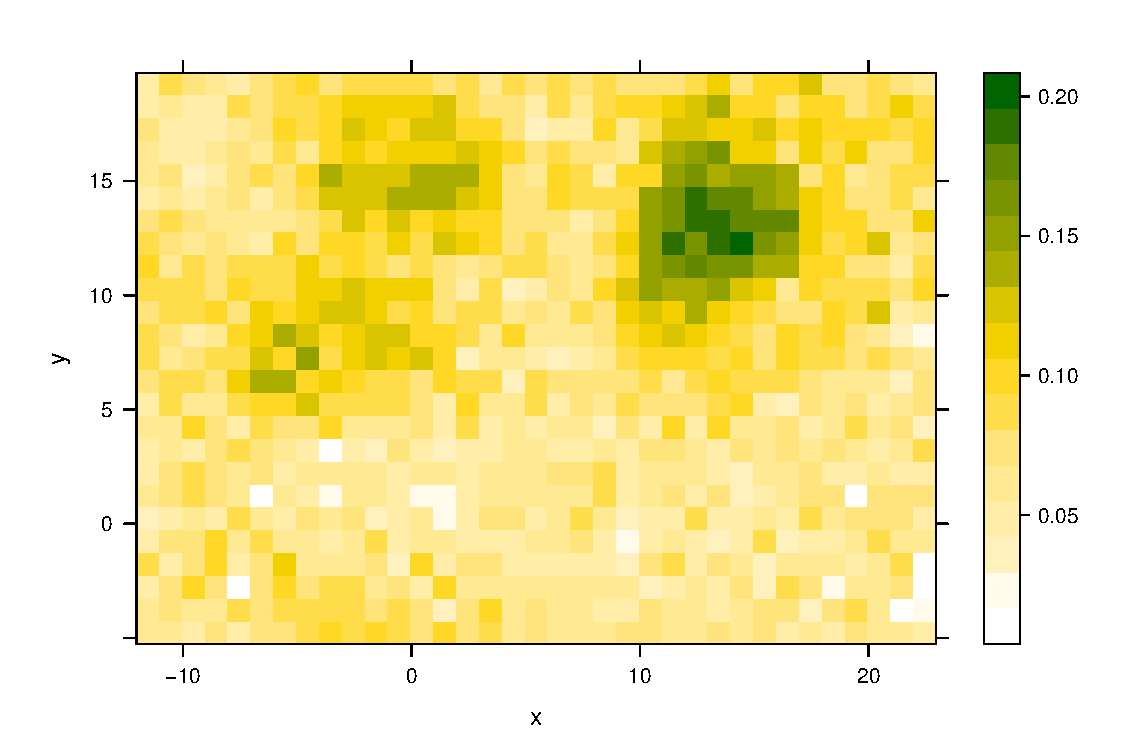
\includegraphics[width=0.495\textwidth]{chondro-fig--DNA}}
\subfloat[\label{fig:DNAsm} Smoothed DNA abundance.]{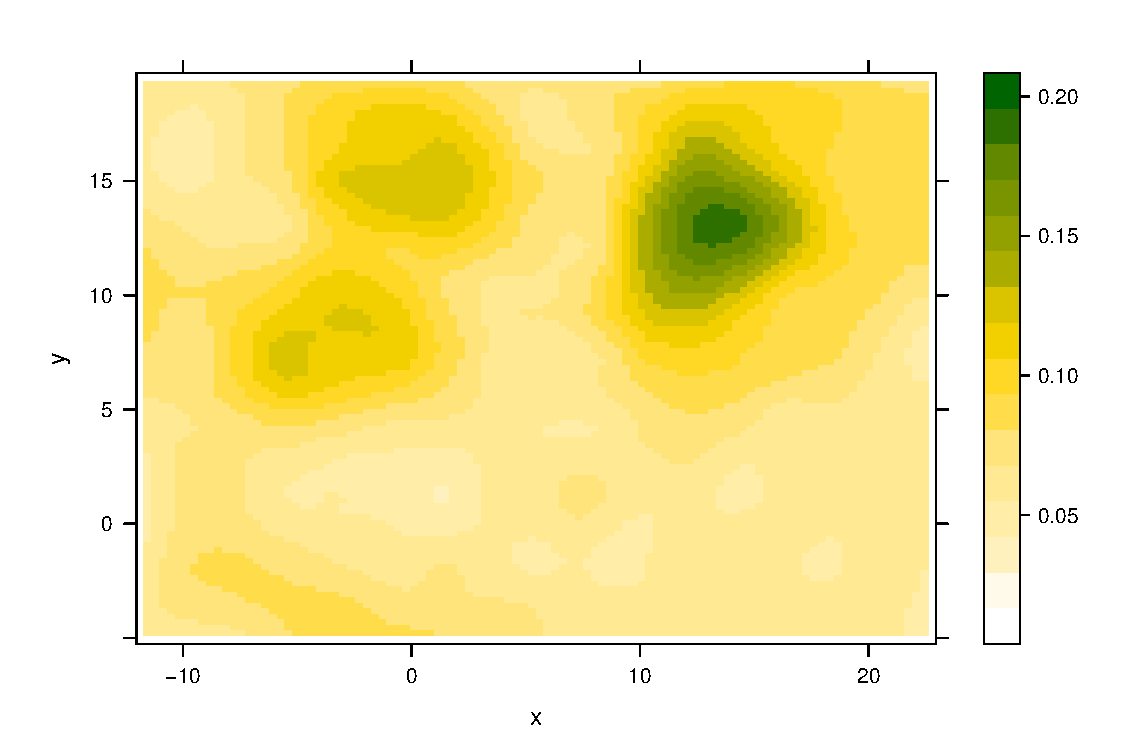
\includegraphics[width=0.495\textwidth]{chondro-fig--DNAsm}}
\caption{False colour map of the DNA band intensities.}
\end{figure}

The result is shown in figure~\ref{fig:DNA}. While the nucleus of
the right cell shows up nicely, only low concentration remainders are detected
of the left cell.

\section{Smoothed False-Colour Maps and Interpolation}
As we plotted only a few selected wavelenths, figure~\ref{fig:DNA} is quite noisy. Smoothing interpolation could help. 
In R, such a smoother is mostly seen as a model, whose predictions are then displayed as smooth map (fig.~\ref{fig:DNAsm}). This smoothing model can be calculated on the fly, 
e.g. by using the \Rfunction{panel.2dsmoother} wrapper provided by \Rpackage{latticeExtra}:

\begin{Schunk}
\begin{Sinput}
> plotmap (chondro[, , c( 728, 782, 1098, 1240, 1482, 1577)],
+        col.regions = DNAcols,
+        panel = panel.2dsmoother, args = list (span = 0.05))
\end{Sinput}
\end{Schunk}

For interpolation (i.e. no smoothing at the available data points), a Voronoi plot  (a.k.a. Delaunay triangulation) is basically a 2d constant interpolation: each point in space has the same z/color value as its closest available point. For a full rectangular grid, this corresponds to the usual square/rectangular pixel plot. With missing points, differences become clear (fig.~\ref{fig:DNAmissing}):

\begin{Schunk}
\begin{Sinput}
> tmp <- sample (chondro[, , c( 728, 782, 1098, 1240, 1482, 1577)], 500)
> plotmap (tmp, col.regions = DNAcols)
\end{Sinput}
\end{Schunk}
\begin{Schunk}
\begin{Sinput}
> plotmap (tmp, col.regions = DNAcols,
+         panel = panel.voronoi, pch = 19, col = "black", cex = 0.1)
\end{Sinput}
\end{Schunk}
\begin{figure}[tbh]
\subfloat[Omitting missing data points.]{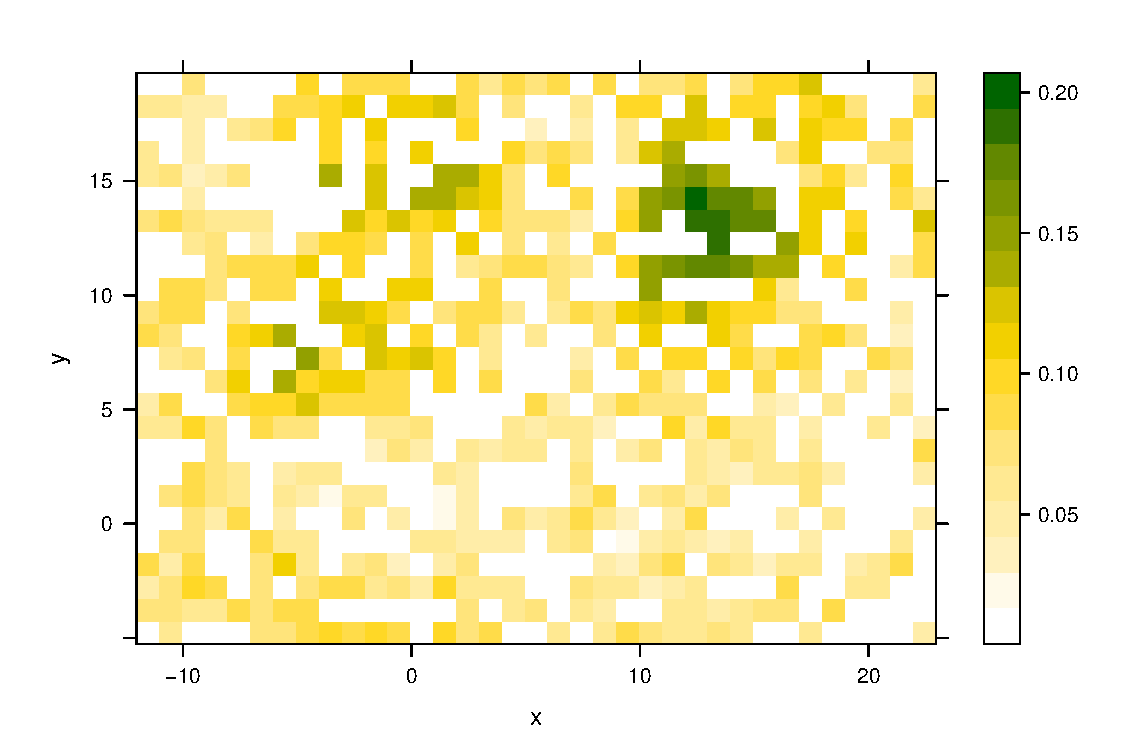
\includegraphics[width=0.495\textwidth]{chondro-fig--DNAmissing}}
\subfloat[Delaunay triangulation / Voronoi plot.]{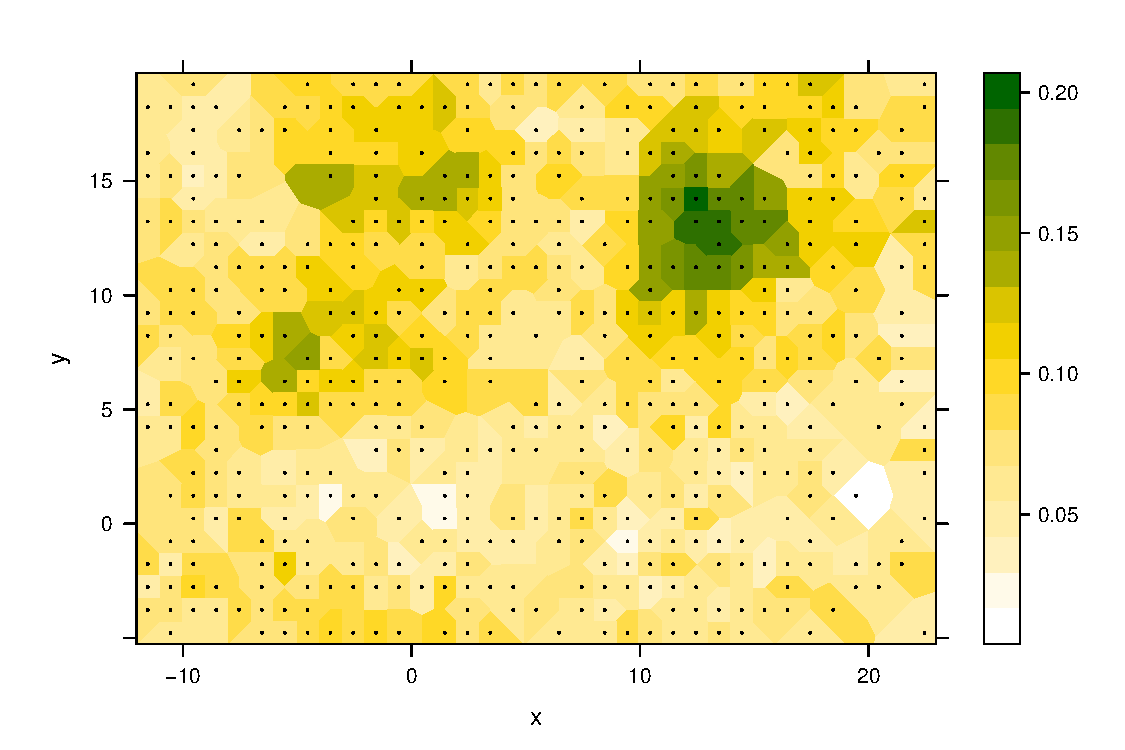
\includegraphics[width=0.495\textwidth]{chondro-fig--DNAvoronoi}}
\caption{\label{fig:DNAmissing} 2d "constant" interpolation with missing values.}
\end{figure}

2d linear interpolation can be done e.g. by the functions provided by package \Rpackage{akima}. However, they do not follow the model-predict paradigm, but instead do directly return an object suitable for base plotting with \Rfunction{image} (\ref{fig:akima}):

\begin{Schunk}
\begin{Sinput}
> if (require ("akima")){
+ 
+ tmp <- rowMeans (chondro[[, , c( 728, 782, 1098, 1240, 1482, 1577)]])
+ chondro.bilinear <- interp (chondro$x, chondro$y, as.numeric (tmp), nx = 100, ny = 100)
+ 
+ image (chondro.bilinear, 
+   xlab = labels (chondro, "x"), ylab = labels (chondro, "y"), 
+   col = DNAcols)
+ } else {
+   plot(NULL, xlim=c(0, 1), ylim=c(0, 1))
+   text(0.5, 0.5, 'Package "akima" is required to create this plot')
+ }
\end{Sinput}
\end{Schunk}
\begin{figure}[tbh]
%\subfloat[Omitting missing data points.]{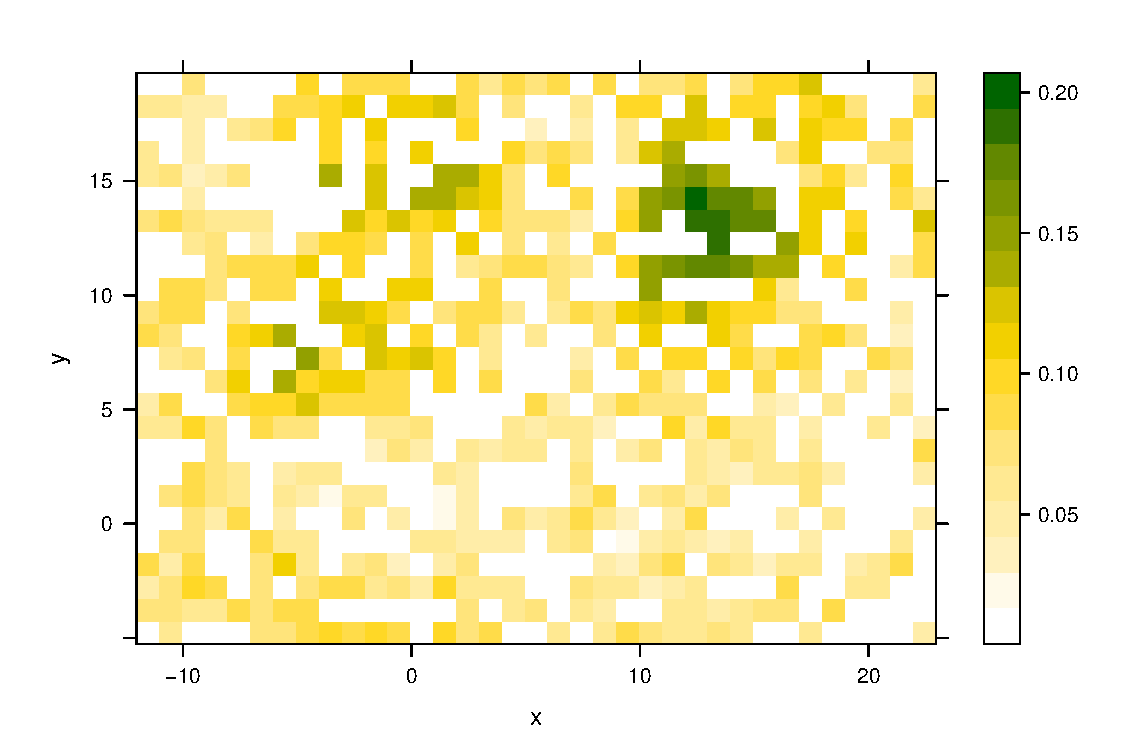
\includegraphics[width=0.495\textwidth]{chondro-fig--DNAmissing}}
%\subfloat[Delaunay triangulation / Voronoi plot.]{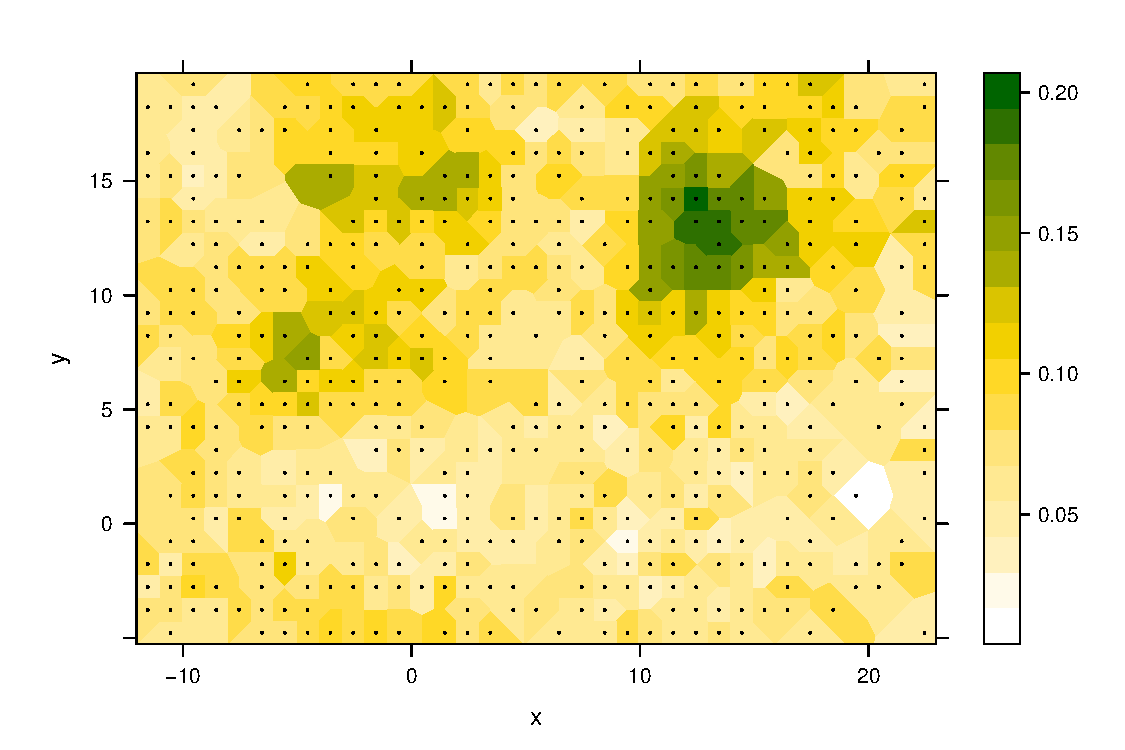
\includegraphics[width=0.495\textwidth]{chondro-fig--DNAvoronoi}}
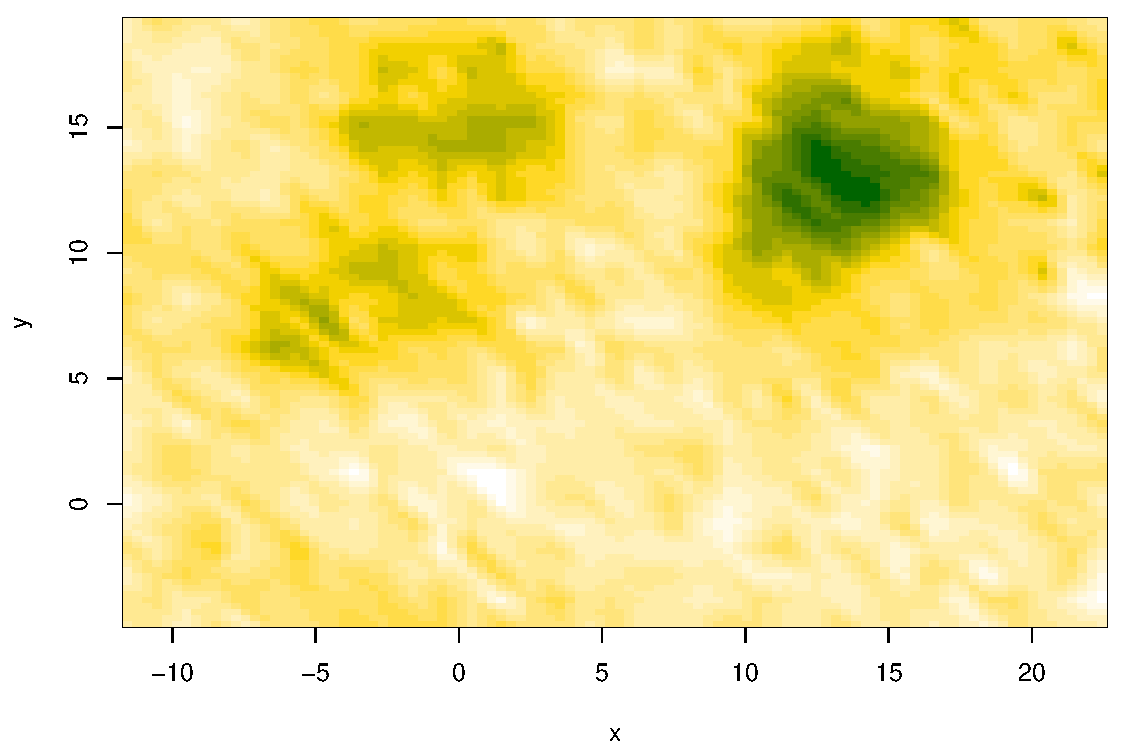
\includegraphics[width=0.495\textwidth]{chondro-fig--DNAinterp}
\caption{\label{fig:akima} 2d interpolation.}
\end{figure}



\section{Saving the data set}
\label{sec:saving-data-set}

Finally, the example data set is put together and saved. In order to keep the package size small,
only a PCA-compressed version with 10 PCs is shipped as example data set of the package.
\begin{Schunk}
\begin{Sinput}
> spectra.to.save$clusters <- factor (NA, levels = levels (chondro$clusters))
> spectra.to.save$clusters[- out] <- chondro$clusters
> pca <- prcomp (spectra.to.save)
> .chondro.scores   <- pca$x      [, seq_len (10)]
> .chondro.loadings <- pca$rot    [, seq_len (10)]
> .chondro.center   <- pca$center
> .chondro.wl       <- wl (chondro)
> .chondro.labels   <- lapply (labels (chondro), as.expression)
> .chondro.extra    <- spectra.to.save$..
> save (.chondro.scores, .chondro.loadings, .chondro.center,
+       .chondro.wl, .chondro.labels, .chondro.extra,
+       file = "chondro-internal.rda")
\end{Sinput}
\end{Schunk}
This is the file distributed with \phy as example data set.

\section*{Session Info}
\begin{footnotesize}
\begin{Schunk}
\begin{Soutput}
R version 3.6.2 (2019-12-12)
Platform: x86_64-pc-linux-gnu (64-bit)
Running under: Ubuntu 18.04.4 LTS

Matrix products: default
BLAS:   /usr/lib/x86_64-linux-gnu/openblas/libblas.so.3
LAPACK: /usr/lib/x86_64-linux-gnu/libopenblasp-r0.2.20.so

locale:
 [1] LC_CTYPE=de_DE.UTF-8       LC_NUMERIC=C               LC_TIME=de_DE.UTF-8       
 [4] LC_COLLATE=de_DE.UTF-8     LC_MONETARY=de_DE.UTF-8    LC_MESSAGES=de_DE.UTF-8   
 [7] LC_PAPER=de_DE.UTF-8       LC_NAME=C                  LC_ADDRESS=C              
[10] LC_TELEPHONE=C             LC_MEASUREMENT=de_DE.UTF-8 LC_IDENTIFICATION=C       

attached base packages:
[1] grid      stats     graphics  grDevices utils     datasets  methods   base     

other attached packages:
[1] akima_0.6-2             latticeExtra_0.6-28     RColorBrewer_1.1-2      hyperSpec_0.99-20200131
[5] ggplot2_3.2.1           lattice_0.20-38        

loaded via a namespace (and not attached):
 [1] Rcpp_1.0.3       magrittr_1.5     tidyselect_0.2.5 munsell_0.5.0    colorspace_1.4-1
 [6] R6_2.4.1         rlang_0.4.2      dplyr_0.8.3      tools_3.6.2      gtable_0.3.0    
[11] withr_2.1.2      deldir_0.1-23    lazyeval_0.2.2   assertthat_0.2.1 tibble_2.1.3    
[16] lifecycle_0.1.0  crayon_1.3.4     purrr_0.3.3      testthat_2.3.1   glue_1.3.1      
[21] sp_1.3-2         compiler_3.6.2   pillar_1.4.2     scales_1.1.0     XML_3.98-1.20   
[26] pkgconfig_2.0.3 
\end{Soutput}
\end{Schunk}
\end{footnotesize}
\end{document}
